%%%%%%%%%%%%%%%%%%%%%%%%%%%%%%%%%%%%%%%%%
% Short Sectioned Assignment
% LaTeX Template
% Version 1.0 (5/5/12)
%
% This template has been downloaded from:
% http://www.LaTeXTemplates.com
%
% Original author:
% Frits Wenneker (http://www.howtotex.com)
%
% License:
% CC BY-NC-SA 3.0 (http://creativecommons.org/licenses/by-nc-sa/3.0/)
%
%%%%%%%%%%%%%%%%%%%%%%%%%%%%%%%%%%%%%%%%%

%----------------------------------------------------------------------------------------
%	PACKAGES AND OTHER DOCUMENT CONFIGURATIONS
%----------------------------------------------------------------------------------------

\documentclass[paper=letter, fontsize=13pt]{article} % A4 paper and 11pt font size

\usepackage[T1]{fontenc} % Use 8-bit encoding that has 256 glyphs
%\usepackage{fourier} % Use the Adobe Utopia font for the document - comment this line to return to the LaTeX default
\usepackage[english]{babel} % English language/hyphenation
\usepackage{amsmath,amsfonts,amsthm} % Math packages

%\usepackage{sectsty} % Allows customizing section commands
%\allsectionsfont{\centering \normalfont\scshape} % Make all sections centered, the default font and small caps
  

\usepackage{color}
\usepackage{listings}
\usepackage{graphicx}
\usepackage{wrapfig}
\usepackage{hyperref}
\usepackage{enumitem}
\usepackage{inconsolata}
\usepackage{framed}

\lstset{language=Haskell}
\definecolor{mygreen}{rgb}{0,0.6,0}
\definecolor{myblue}{rgb}{0.2,0.2,0.8}
\definecolor{mymauve}{rgb}{0.58,0,0.82}

\lstset{ %
%  numbers=left,
  basicstyle=\ttfamily,
  showstringspaces=false,
  backgroundcolor=\color{white},   % choose the background color
%  breaklines=true,                 % automatic line breaking only at whitespace
  captionpos=b,                    % sets the caption-position to bottom
  commentstyle=\color{mygreen},    % comment style
  escapeinside={(*}{*)},          % if you want to add LaTeX within your code
  keywordstyle=\color{mymauve},       % keyword style
}

% Add your keywords here, and have this in a separate file
% and include it in your preamble
\lstset{emph={%  
    DECR,EQL,TRUE, FALSE, ITE, NOT, AND, OR, PAIR, FST, SND, ZERO, ONE,% 
    TWO, THREE, FOUR, FIVE, INC, ADD, MUL, ISZ, GET, APPEND, REVERSE, FIX, EMPTY, S\_GET, CONVERT, LENGTH%
    },emphstyle={\bfseries}%
}%


\usepackage[margin=1in]{geometry}
%\usepackage{fancyhdr} % Custom headers and footers
%\pagestyle{fancyplain} % Makes all pages in the document conform to the custom headers and footers
%\fancyhead{} % No page header - if you want one, create it in the same way as the footers below
%\fancyfoot[L]{} % Empty left footer
%\fancyfoot[C]{} % Empty center footer
%\fancyfoot[R]{\thepage} % Page numbering for right footer
%\renewcommand{\headrulewidth}{0pt} % Remove header underlines
%\renewcommand{\footrulewidth}{0pt} % Remove footer underlines
%\setlength{\headheight}{13.6pt} % Customize the height of the header


\numberwithin{equation}{section} % Number equations within sections (i.e. 1.1, 1.2, 2.1, 2.2 instead of 1, 2, 3, 4)
%\numberwithin{figure}{section} % Number figures within sections (i.e. 1.1, 1.2, 2.1, 2.2 instead of 1, 2, 3, 4)
%\numberwithin{table}{section} % Number tables within sections (i.e. 1.1, 1.2, 2.1, 2.2 instead of 1, 2, 3, 4)

%\setlength\parindent{0pt} % Removes all indentation from paragraphs - comment this line for an assignment with lots of text

%----------------------------------------------------------------------------------------
%	TITLE SECTION
%----------------------------------------------------------------------------------------

\newcommand{\horrule}[1]{\rule{\linewidth}{#1}} % Create horizontal rule command with 1 argument of height
\newif\ifshowanswers\showanswerstrue

\title{\vspace{-2em} 	
\normalfont \normalsize 
%\horrule{0.5pt} \\[0.4cm] % Thin top horizontal rule
{\huge CSE 116, Fall 2019 Midterm} \\ % The assignment title
\horrule{2pt} \\[0.5cm] % Thick bottom horizontal rule
}
\date{\vspace{-4em}} % Today's date or a custom date

\begin{document}

\maketitle % Print the title

%----------------------------------------------------------------------------------------
%	PROBLEM 1
%----------------------------------------------------------------------------------------

% TODO : Random list?
% https://tex.stackexchange.com/questions/96645/random-shuffle-itemize
\begin{center}
 {\Large
\begin{tabular}{|c|c|c|}
\hline
\textbf{Section} & \textbf{Points} & \textbf{Score} \\
\hline
Part I     & 40 points  & \\
\hline
Part II   &  56 points &   \\
\hline
 \textbf{Total} & 96 points &   \\
\hline
\end{tabular}
}

\end{center}
\large 


\paragraph{\textbf{ Instructions} }
\begin{itemize}

\item \textbf{You have 95 minutes to complete this exam.}

\item This exam is \textbf{closed book}.  You may use one double-sided
page of notes, but no other materials.

\item Avoid seeing anyone else's work or allowing yours to be seen.

\item Do not communicate with anyone but an exam proctor.

\item To ensure fairness (and the appearance thereof),
  \textbf{proctors will not answer questions about the content of the exam}. If you are unsure 
  of how to interpret a problem description, state your interpretation clearly and concisely. 
  \textit{Reasonable interpretations} will be taken into account by graders.

\end{itemize}

\bigskip
\bigskip
\bigskip
\bigskip
\bigskip
\bigskip
\bigskip
\bigskip
\bigskip
\bigskip
\bigskip
\bigskip
\bigskip
\bigskip
\bigskip
\bigskip
\noindent NAME: \verb|____________________________________________________| \\
\bigskip\\ 
\bigskip\\
CruzID: \verb|_______________________________| @ucsc.edu

\newpage
\noindent {\Huge \textbf{Part I: Lambda calculus}}

\bigskip

\begin{enumerate} 
\item \textbf{[16pts]} Use $\beta$-reductions to evaluate the following lambda term to a normal form. \\
\bigskip
\bigskip
\begin{enumerate}[label=(\Alph*)]
\item {\Large
\verb|((\p q -> p q) ((\x -> x) (\a b -> a))) (\k -> k)|
}
\ifshowanswers
\begin{itemize}
\item \verb|=b> (\q -> ((\x -> x) (\a b -> a)) q) (\k -> k)|
\item \verb|=b> ((\x -> x) (\a b -> a)) (\k -> k)|
\item \verb|=b> (\a b -> a) (\k -> k)|
\item \verb|=b> (\b k -> k)|
\end{itemize}
Rubric:
\begin{itemize}
\item 0 pts : no attempt or nothing correct.
\item 1 pts : anything correct (e.g., one reduction)
\item 2-3 pts : more than one thing correct (e.g., two reductions), few things incorrect
\item 4 pts : almost correct, but one smallish error
\item 5 pts : completely correct
\end{itemize}
\else
\bigskip
\bigskip
\bigskip
\bigskip
\bigskip
\bigskip
\bigskip
\bigskip
\bigskip
\bigskip
\bigskip
\bigskip
\bigskip
\bigskip
\bigskip
\bigskip
\bigskip
\bigskip
\bigskip
\bigskip
\bigskip
\bigskip
\fi

\item {\Large
\verb|(\x y -> (y x)) (\p q -> p) (\i -> i) (\j -> j)|
}
\ifshowanswers
\begin{itemize}
\item \verb|=b> (\y -> y (\p q -> p)) (\i -> i) (\j -> j)|
\item \verb|=b> (\i -> i) (\p q -> p) (\j -> j)|
\item \verb|=b> (\p q -> p) (\j -> j)|
\item \verb|=b> \q -> (\j -> j)|
\end{itemize}
Rubric:
\begin{itemize}
\item 0 pts : no attempt or nothing correct.
\item 1 pts : anything correct (e.g., one reduction)
\item 2-3 pts : more than one thing correct (e.g., two reductions), few things incorrect
\item 4 pts : almost correct, but one smallish error
\item 5 pts : completely correct
\end{itemize}
\fi
\end{enumerate}
\newpage

\item \textbf{[8pts]}  For each bound occurrence of a variable in the following lambda terms, 
draw an arrow pointing to its binder. For each free occurrence, draw a circle around the variable.

\bigskip
\bigskip
\bigskip

\begin{enumerate}[label=(\Alph*)]
\item {\Large
  \verb|(\a ->  b  (\b  a -> a  b))|
}
\ifshowanswers
Rubric:
\begin{itemize}
\item 0 pts : no attempt or nothing correct.
\item 1 pts : anything correct 
\item 2 pts : more than one thing correct, few things incorrect
\item 3 pts : completely correct
\end{itemize}
\else
\bigskip
\bigskip
\bigskip
\fi

\item {\Large
  \verb|(\p  q  r  -> (p  (\q  p  -> (r  q))) (q  p))|
}
\end{enumerate}

\bigskip
\bigskip
\bigskip

\item \textbf{[16pts]}  
Fill in a lambda calculus expression for each blank in the program
below to define a function \texttt{PROD} where \texttt{(PROD n)} returns 
the product of numbers between
$n$ and one. You may use any of the functions defined on the Lambda
Calculus Cheat Sheet on the back page.  Any other helper functions you
must define yourself. Your implementation may assume that \texttt{PROD} is never
called with \texttt{ZERO}.

\begin{verbatim}
let PROD1 = \f n -> ITE _____(A)_______
                        _____(B)_______
                        _____(C)_______
                      
let PROD  = ______(D)_______
\end{verbatim}
\begin{enumerate}[label=(\Alph*)]
   \item 
     \ifshowanswers 
      (3pts) \verb|(EQL n ONE)| or \verb|(EQL ONE n)|  (parens optional).  Minor deduction (.5) for more complicated but correct answer.  Full credit if it is just the negation (i.e., using NOT)
     \else
           \bigskip
           \bigskip
           \bigskip
           \bigskip
           \bigskip
           \bigskip
     \fi
   \item
     \ifshowanswers 
       (3pts) \verb|ONE|  or \verb|n| 
     \else
           \bigskip
           \bigskip
           \bigskip
           \bigskip
           \bigskip
           \bigskip
     \fi
   \item
     \ifshowanswers 
      (5pts) \verb|MULT n (f (DECR n))|. Full credit  requires correct operation (MULT), correct use of recursive call (f), and correct argument to f (DECR n), roughly equal weight.  Minor deduction (.5) for more complicated answer or other small errors.
     \else
           \bigskip
           \bigskip
           \bigskip
           \bigskip
           \bigskip
           \bigskip
     \fi
   \item 
     \ifshowanswers 
     (5pts) \verb|FIX PROD1| . Half credit at least if FIX is applied to PROD1 in some way.
     \else
           \bigskip
           \bigskip
           \bigskip
           \bigskip
           \bigskip
           \bigskip
     \fi
\end{enumerate}

\newpage
\noindent {\Huge \textbf{Part II: Haskell}}
\bigskip
\bigskip
\bigskip
\item \textbf{[5pts]} What does the following Haskell program evaluate to?
\begin{lstlisting}
let f = (\x -> \y -> x + y)
    g = f 5 
    h = \f n -> f (f n)
in 
  h g 3
\end{lstlisting}
  \begin{enumerate}
    \item Type Error
    \item \verb|8|
    \item \verb|13|
    \item \verb|\f -> f (f 8)|
    \item \verb|16|
  \end{enumerate}
\ifshowanswers
\textbf{Answer: C}
\fi
  
\bigskip
\bigskip
\bigskip
\bigskip
\bigskip
  
\item \textbf{[5pts]} What is the most general type of the Haskell function \texttt{foo}?
\begin{lstlisting}
foo bar (x, y)
  | bar x      =  y ++ y
  | otherwise  =  y 
\end{lstlisting}
    \begin{enumerate} 
         \item \verb|(a -> b) -> (a,b) -> [b]|
         \item \verb|(String -> Bool) -> (String, String) -> String|
         \item \verb|(a -> Bool) -> (a, a) -> [a]|
         \item \verb|(Bool -> a) -> [b] -> [b]|
         \item \verb|(a -> Bool) -> (a, [b]) -> [b]|
     \end{enumerate}
\ifshowanswers
  \textbf{Answer: E}
\fi

\newpage
For the following questions, consider the data types defined below.
\begin{lstlisting}

data TrickOrTreat = Trick Prank | Treat Candy 

data Prank = Prank { desc :: String, legal :: YNM }

data YNM = Yes | No | Maybe

data Candy = Candy { pieces :: Int, kind :: Kind, rating :: Int}

data Kind = Chocolate | HardCandy | Gummies
\end{lstlisting}

\item \textbf{[21pts]} A \texttt{case} expression is \textit{exhaustive} if all possible values are matched
by at least one pattern. A pattern is \textit{overlapping} if previous patterns match all values it matches.
Assume \texttt{t} has type \texttt{TrickOrTreat} and do the following:
\begin{itemize}
  \item For each pattern in each \texttt{case}, provide a value that matches on the pattern.
  \item If the pattern is overlapped by previous patterns, write ``N/A''.
  \item Determine if the \texttt{case} expression is exhaustive and circle \texttt{Exhaustive} or \texttt{Non-exhaustive} as appropriate.
  \item For non-exhaustive \texttt{case} expressions, write a value that does not match any of its patterns.
\end{itemize}
\begin{enumerate}

\item 
\begin{lstlisting}
                            case t of


_______________________       Trick (Prank _ Yes) -> ()


_______________________       Trick (Prank d No) -> ()


_______________________       Trick _ -> ()


_______________________       _ -> ()


_______________________    [ Exhaustive  /  Non-exhaustive ]
\end{lstlisting}
\newpage

\item
\begin{lstlisting}
                           case t of


_______________________      Treat (Candy _ k r) | r > 3 -> ()


_______________________      Trick (Prank d l) -> ()


_______________________      Treat c | (rating c) < 3 -> ()


_______________________    [ Exhaustive  /  Non-exhaustive ]
\end{lstlisting}
\bigskip
\bigskip
\bigskip

\item
\begin{lstlisting}
                           case t of
                           
                           
_______________________      Treat c -> ()
                           
                           
_______________________      Treat (Candy n Chocolate r) -> ()  
                           
                           
_______________________      Trick p -> ()


_______________________    [ Exhaustive  /  Non-exhaustive ]
\end{lstlisting}
           \bigskip
           \bigskip
           \bigskip
           \bigskip

\item
\begin{lstlisting}
                       case t of


____________________     Trick (Prank "snakes on plane" No) -> ()


____________________     Treat (Candy 99 Gummies r) -> ()


____________________     Treat _ -> ()


____________________    [ Exhaustive  /  Non-exhaustive ]
\end{lstlisting}

\end{enumerate}

\newpage
\item Consider a binary search tree where each internal node has a value $i$ and two child subtrees.  
The left child contains all nodes with values less than or equal to $i$, and the
right child contains all nodes with values strictly greater than $i$.  

\begin{figure}[h]
  \begin{center}
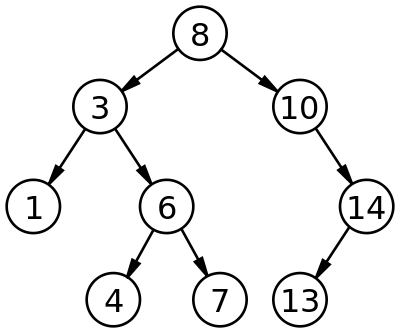
\includegraphics[width=0.3\textwidth]{bst}
\caption{A binary search tree}
\label{fig:bst}
\end{center}
\end{figure}

\begin{enumerate}[label=(\Alph*)]
  \item \textbf{[5pts]} Using the following ADT, create a \texttt{Tree} that represents the binary search tree in Figure~\ref{fig:bst}.
\begin{lstlisting}
data Tree =  Leaf | Node Int Tree Tree
\end{lstlisting}
    \ifshowanswers 
\begin{verbatim}
(Node 8 (Node 3 (Node 1 Leaf Leaf) 
                (Node 6 (Node 4 Leaf Leaf) (Node 7 Leaf Leaf))) 
        (Node 10 Leaf (Node 14 (Node 13 Leaf Leaf) Leaf)))| 
\end{verbatim}
    \else
     \bigskip
     \bigskip
     \bigskip 
     \bigskip
     \bigskip 
     \bigskip
     \bigskip
     \bigskip 
     \bigskip
     \bigskip
    \fi
 
  \item \textbf{[10pts]} Define the function \texttt{max}, which returns the highest value in a binary search tree represented by a \texttt{Tree} value, or 0 if the tree is empty.  
            For example, if \texttt{t} is the tree in Figure~\ref{fig:bst}, then \texttt{max t} evaluates to 14.  Full credit requires an efficient traversal
            of the tree (e.g., not an exhaustive one). You may define helper functions if desired, but you may not use any library functions except \texttt{==}, \texttt{>=}, or \texttt{<=}.
\begin{lstlisting}
max :: Tree -> Int
\end{lstlisting}
    \ifshowanswers 
\begin{lstlisting}
max Leaf = 0
max (Node n t1 Leaf) = n
max (Node n t1 t2) = max t2
\end{lstlisting}
    \else
     \bigskip 
     \bigskip 
     \bigskip
     \bigskip
     \bigskip
     \bigskip
     \bigskip
     \bigskip
     \bigskip 
     \bigskip
     \bigskip 
     \bigskip
     \bigskip
    \fi


  \item \textbf{[10pts]} Define the function \texttt{contains}, which returns \texttt{True} if a number \texttt{n} is contained in a binary search tree \texttt{t}.
            For example, if \texttt{t} is the tree in Figure~\ref{fig:bst}, then \texttt{contains 7 t} returns \texttt{True}, but \texttt{contains 5 t} returns \texttt{False}.
            Full credit requires an efficient traversal of the tree (e.g., not an exhaustive one). You may define helper functions if desired, but you may not use any 
            library functions except \texttt{==}, \texttt{>=}, or \texttt{<=}. 
\begin{lstlisting}
contains :: Int -> Tree -> Bool
\end{lstlisting}
    \ifshowanswers 
\begin{lstlisting}
contains n Leaf = False
contains n (Node m t1 t2) | (n == m) = True
                          | otherwise = if (n <= m) then 
                                          (contains n t1) 
                                        else 
                                          (contains n t2)
\end{lstlisting}
    \else
     \bigskip 
     \bigskip 
     \bigskip
     \bigskip
     \bigskip
     \bigskip
     \bigskip
     \bigskip
     \bigskip 
     \bigskip
     \bigskip 
     \bigskip
     \bigskip
    \fi

\end{enumerate}
\end{enumerate}

\newpage
\[ \]
\newpage
\section{Lambda calculus cheat sheet}
\begin{lstlisting}
-- Booleans --------------------------------
let TRUE =\x y -> x
let FALSE = \x y -> y
let ITE = \b x y -> b x y
let NOT = \b x y -> b y x
let AND = \b1 b2 -> ITE b1 b2 FALSE 
let OR = \b1 b2 -> ITE b1 TRUE b2

-- Numbers ---------------------------------
let ZERO = \f x-> x
let ONE = \f x -> f x 
let TWO = \f x -> f (f x) 
let THREE = \f x -> f (f (f x))
let FOUR = \f x -> f (f (f (f x))
let FIVE = \f x -> f (f (f (f (f x))

-- Arithmetic ------------------------------
let INC   = \n f x -> f (n f x)
let ADD   = \n m -> n INC m 
let MUL   = \n m -> n (ADD m) ZERO
let ISZ   = \n ->   -- return TRUE if n == 0 --
let DECR  = \n ->   -- decrement n by one --  
let EQL   = \a b -> -- return TRUE if a == b, otherwise FALSE --

-- Recursion -------------------------------
let FIX = \stp -> (\x -> stp (x x)) (\x -> stp (x x))
\end{lstlisting}

\end{document}
